\pagebreak
\section{Erste Hilfe}
Grundsätzlich gilt auch in Arma: \textbf{Eigenschutz geht vor Fremdschutz!}. Bevor ihr eurem Buddy oder einem Kameraden helft, stellt sicher, dass ihr dies auch gefahrlos tun könnt! Ansonsten liegt noch jemand verwundet in der Gefahrenzone!\\
Folgende Schritte sind zu tun:
\begin{enumerate}
	\item Sichern und Bergen des Verwundeten (Rauchgranaten einsetzen!)\\
			Eigenschutz geht vor! Erst die Umgebung sichern, dann den Verletzten bergen! 
	\item Bewusstsein und Puls checken (ggf. CPR anwenden lassen!)
	\item Verletzungsgrad feststellen
	\item \textbf{Melden: Verletzungsgrad, Position, weitere Angaben!}
	\item Blutungen stillen! (Gliedmaßen abbinden, Verletzungen versorgen) \newline
	 >>Avulsions<< (Abriss) und >>Velocity wounds<< (Balistisches Traum) werden mit Packing Bandage (Mullbinde) behandelt, alles andere Verletzungen mit der elastic Bandage (elastische Bandage)
	\item ggf. Sanitäter/MedEvac anfordern
	\item Patienten stabil halten, bis Sanitäter eintrifft oder Patient transportiert werden kann.
	\item Falls nötig, Patient verlegen
\end{enumerate}
Den Anweisungen des Sanitätspersonals ist Folge zu leisten! Falls nötig, ist der Patient selbstständig zu einer Verwundetensammelstelle zu verlegen.
Zur Veranschaulichung oder zum Ausdruck kann folgendes Flussdiagramm behilflich sein.

\begin{figure}[htbp]
		\centering
		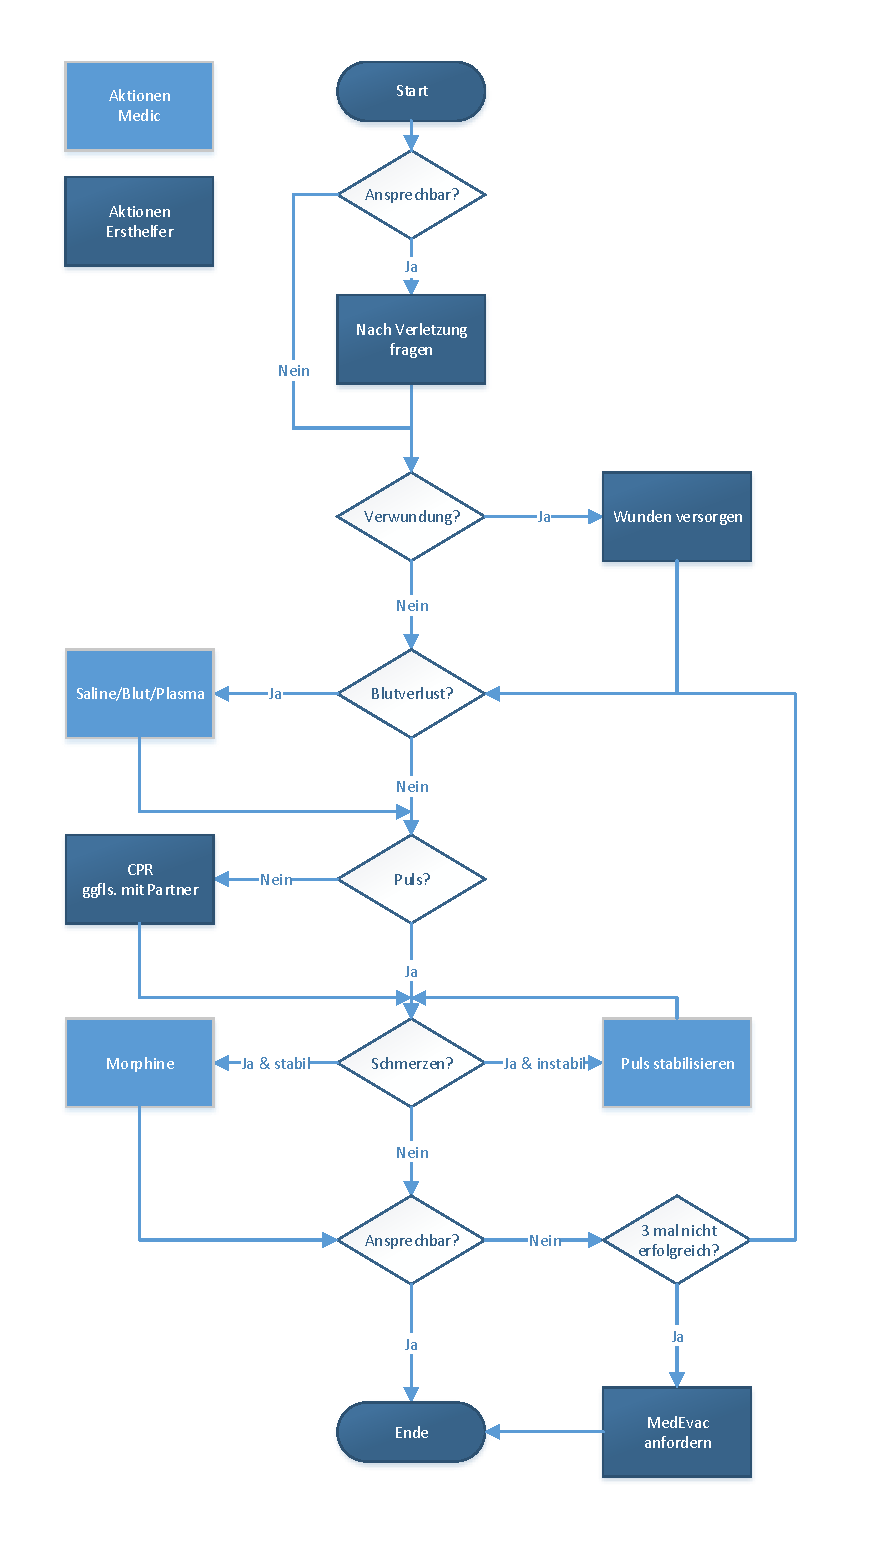
\includegraphics[height=0.95\textheight]{../img/basic/erste_hilfe/ersthelfer}
		\caption{Erste Hilfe im TTT}
\end{figure}
